\titleformat {\chapter} {\normalfont\huge\bfseries\color{black}}   {\thechapter}{10pt}{\huge} 
\chapter {Simulation Results}

%% ================================
%% \input{Advice-on-Chapter-4}
%% ================================
	
\section{The Parametric Equations}
%% \label{sec:4.1-CNC-Research-Machine}

The images of the UMP 3-axis CNC research machine for our previous work are provided in next three figures. It is an experimental CNC router-type, that instead of a tool cutter, uses a pen to create drawings on paper in the X-Y plane. The Z-axis motion is used to raise and lower the pen. As a consequence, circular arc (G02, G03 G-Code) moves are applicable to the X and Y axes only, while linear (G01 G-Code) moves are applicable to all three X, Y and Z axes.  
\vspace*{1\baselineskip}
		
\pagebreak
%% ================================================
\begin{table}[ht]
	\begin{center}
		\begin{tabular}[top]{ |p{16.0 cm}| }
			\rowcolor{LIGHTCYAN}			
			\hline \multicolumn{1}{|c|}{\textbf{Part 1/5 Teardrop and Butterfly parametric curves}} \\ [1.0ex]
	
			\hline \textbf{\textbf{Teardrop parametric curve}}\\
			 \begin{eqnarray}
			 x(u) & = & - 150u + 450u^2 - 300u^3 \nonumber \\   
			 y(u) & = & - 150u + 150u^2 \nonumber \\
			 u & \in & [0.0, 1.0] \nonumber
			\end{eqnarray}
		
			 Closed loop\\
			 Overall Single loop\\
			 Reflection x-axis: non-symmetrical\\
			 Reflection y-axis: symmetrical\\
			 \frame{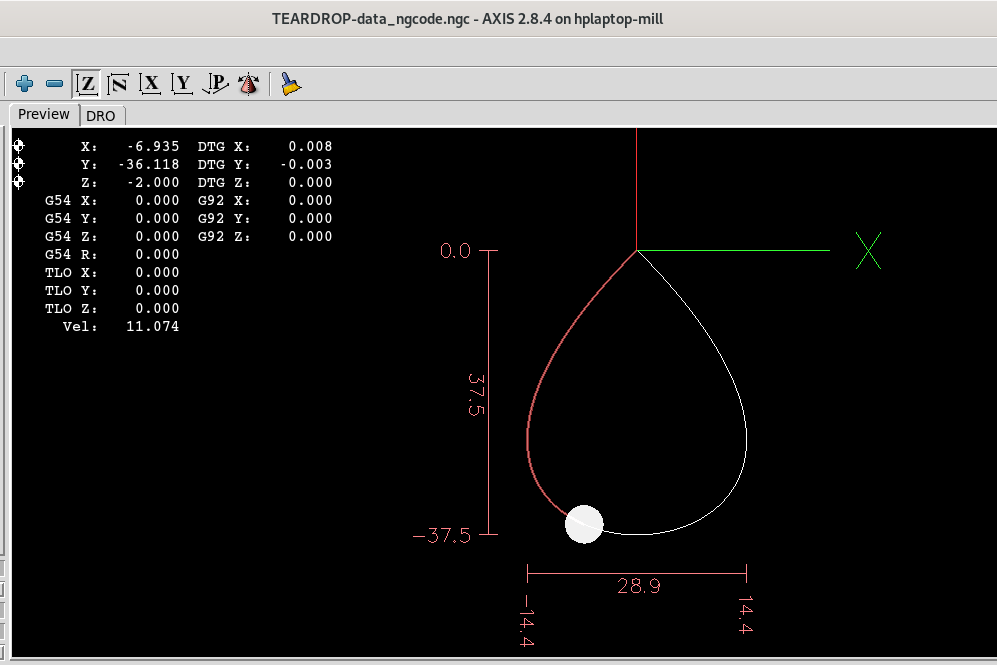
\includegraphics[width=0.565\textwidth]{./07-images/img-Ch5/TEARDROP-Axis.png}}
			 \frame{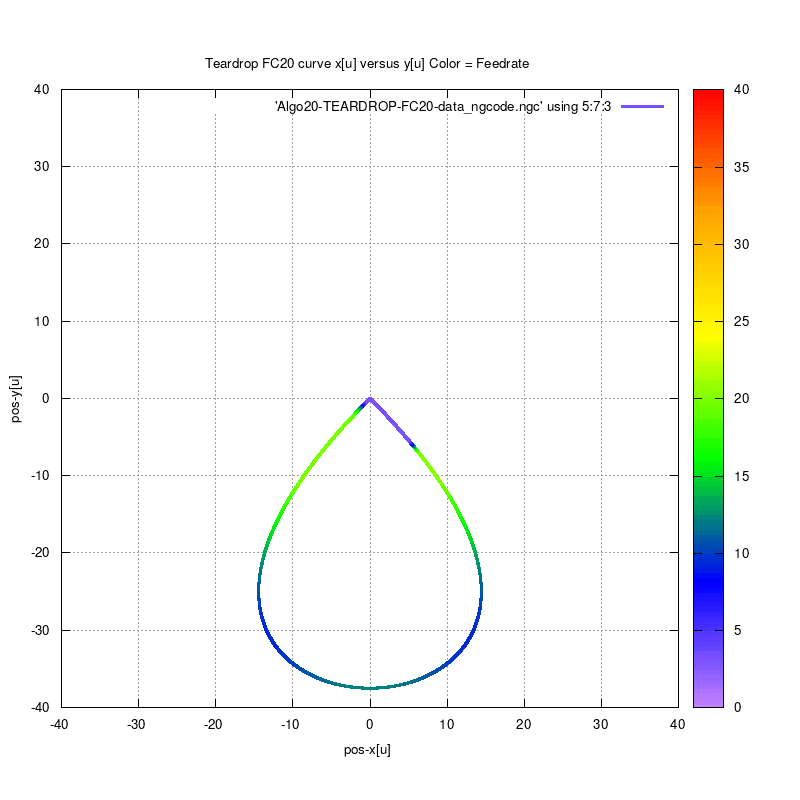
\includegraphics[width=0.38\textwidth]{./07-images/img-Ch5/TEARDROP-Feedrate.png}}\\
			
			\hline \textbf{Butterfly parametric curve}\\
			\begin{eqnarray}
				x(u) & = & \sin(u) \left [ e^{\cos(u)} - 2\cos(4u) - (\sin(u/12))^5 \right] \nonumber \\
				y(u) & = & \cos(u) \left [ e^{\cos(u)} - 2\cos(4u) - (\sin(u/12))^5 \right] \nonumber \\
				u & \in & [0.0, 2\pi] \nonumber
			\end{eqnarray}
			      
			
			Closed loop\\
			Overall Multiple loops\\
			Reflection x-axis: non-symmetrical\\
			Reflection y-axis: symmetrical\\
			\frame{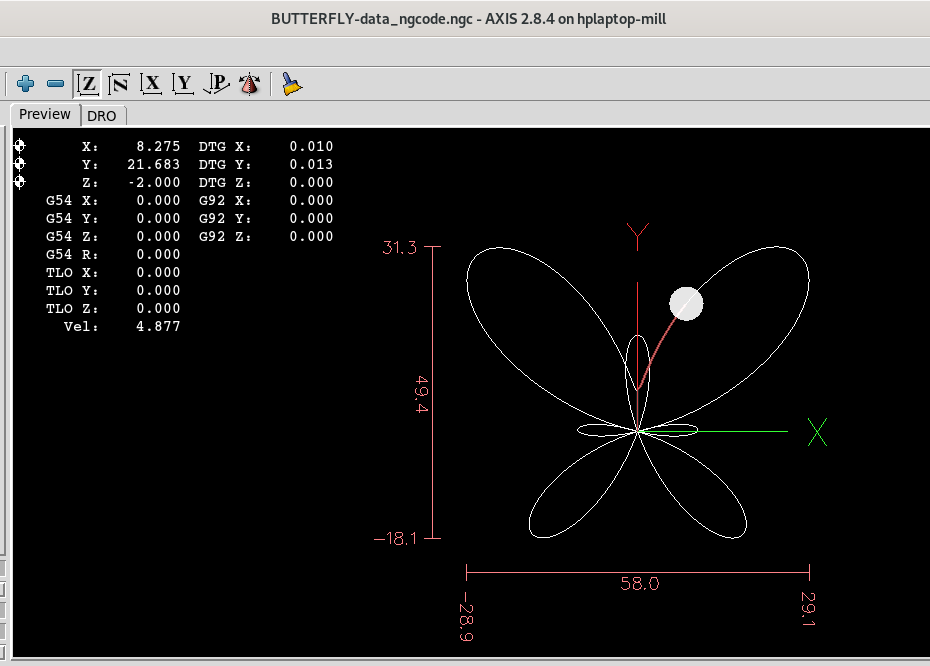
\includegraphics[width=0.56\textwidth]{./07-images/img-Ch5/BUTTERFLY-Axis.png}}
            \frame{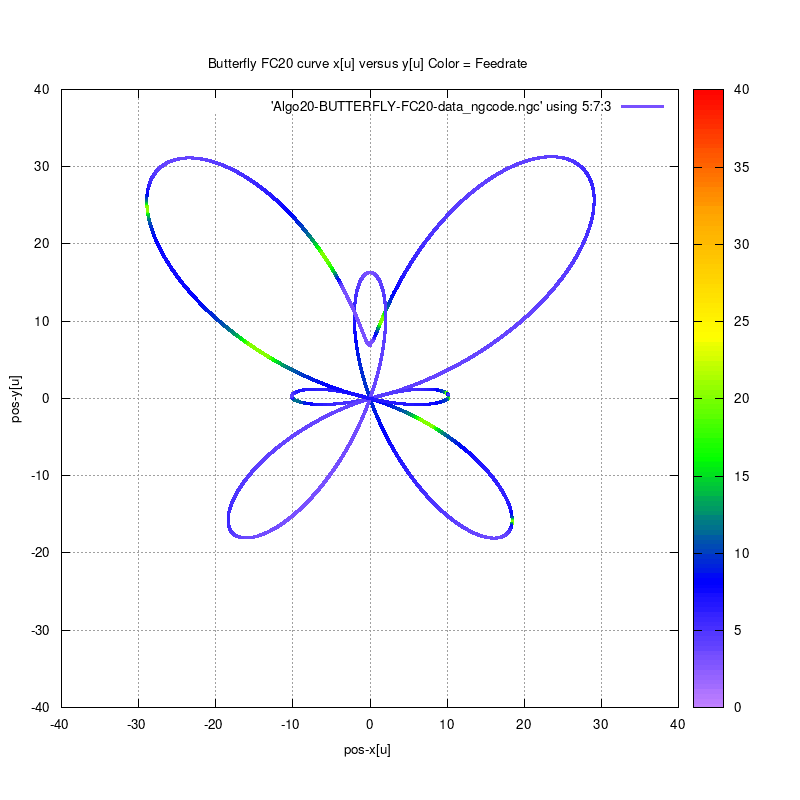
\includegraphics[width=0.40\textwidth]{./07-images/img-Ch5/BUTTERFLY-Feedrate.png}}\\

			\hline
		\end{tabular}
		%% \caption{Equations and dimensions of Teardrop and Butterfly curves}		
		\label{table:Part1of5 Equations and dimensions of the parametric curves}
	\end{center}
\end{table}  

\pagebreak

%% ================================================
\begin{table}[ht]
	\begin{center}
		\begin{tabular}[top]{ |p{16.0 cm}| }
			\rowcolor{LIGHTCYAN}			
			\hline \multicolumn{1}{|c|}{\textbf{Part 2/5 Ellipse and Skewed-Astroid parametric curves}} \\ [1.0ex]
			
			\hline \textbf{\textbf{Ellipse parametric curve}}\\
			\begin{eqnarray}
				x(u) & = & - 150u + 450u^2 - 300u^3 \nonumber \\   
				y(u) & = & - 150u + 150u^2 \nonumber \\
				u & \in & [0.0, 1.0] \nonumber
			\end{eqnarray}
			
			Closed loop\\
			Overall Single loop, smooth convex curves\\
			Reflection x-axis: symmetrical\\
			Reflection y-axis: symmetrical\\
			\frame{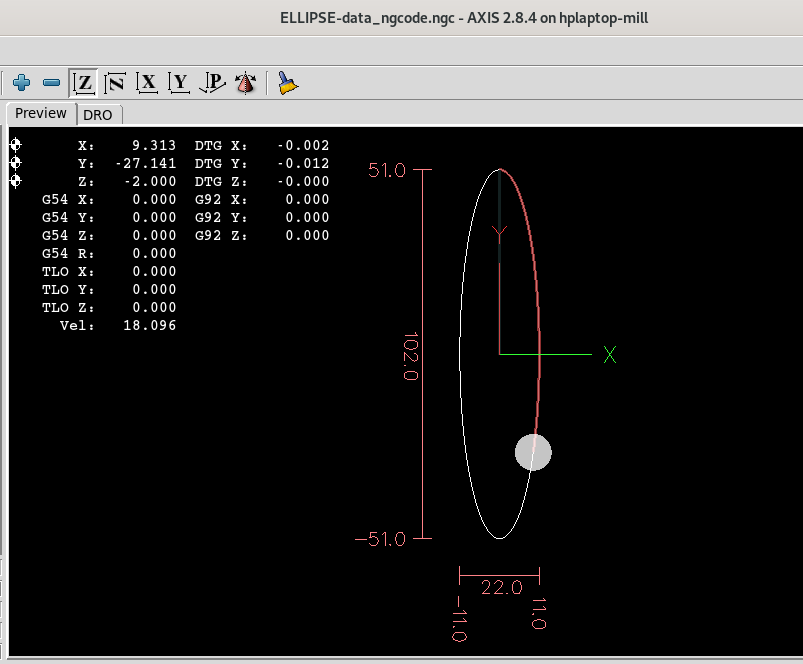
\includegraphics[width=0.51\textwidth]{./07-images/img-Ch5/ELLIPSE-Axis.png}}
			\frame{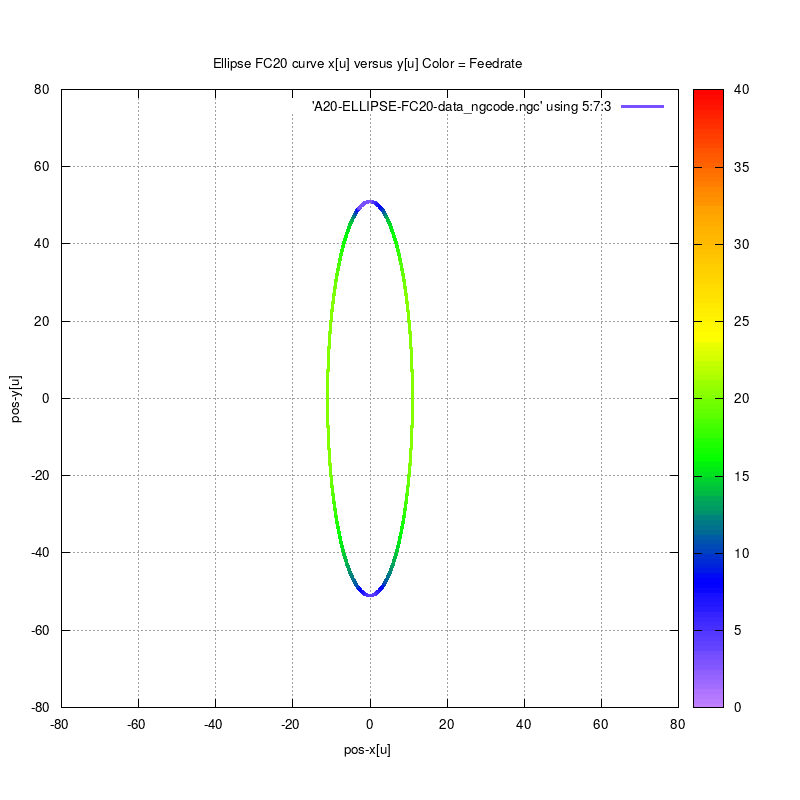
\includegraphics[width=0.42\textwidth]{./07-images/img-Ch5/ELLIPSE-Feedrate.png}}\\
			
			\hline \textbf{Skewed-Astroid parametric curve}\\
			\begin{eqnarray}
				x(u) & = & \sin(u) \left [ e^{\cos(u)} - 2\cos(4u) - (\sin(u/12))^5 \right] \nonumber \\
				y(u) & = & \cos(u) \left [ e^{\cos(u)} - 2\cos(4u) - (\sin(u/12))^5 \right] \nonumber \\
				u & \in & [0.0, 2\pi] \nonumber
			\end{eqnarray}
			
			
			Closed loop\\
			Overall Single loop, 4 cusps and 4 concave curves \\
			Reflection x-axis: symmetrical\\
			Reflection y-axis: symmetrical\\
			\frame{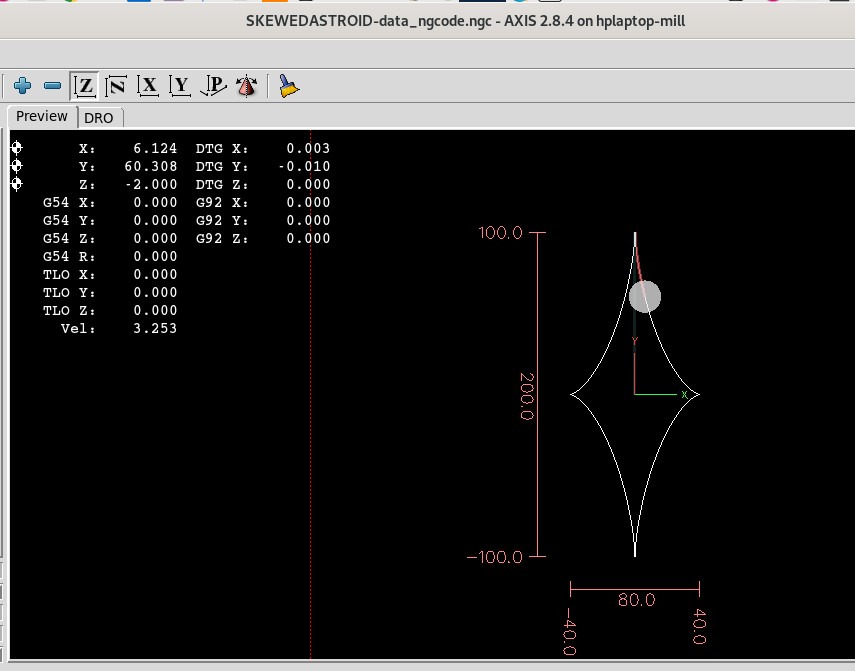
\includegraphics[width=0.51\textwidth]{./07-images/img-Ch5/SKEWED-ASTROID-Axis.png}}
			\frame{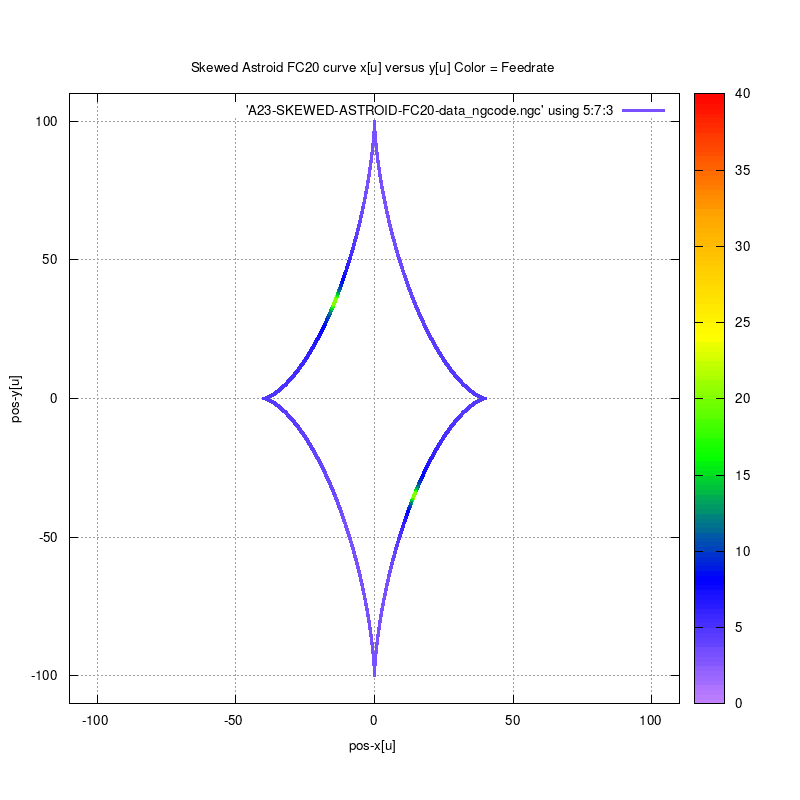
\includegraphics[width=0.40\textwidth]{./07-images/img-Ch5/SKEWED-ASTROID-Feedrate.png}}\\
			
			\hline
		\end{tabular}
		%% \caption{Equations and dimensions of Teardrop and Butterfly curves}		
		\label{table:Part2of5 Equations and dimensions of the parametric curves}
	\end{center}
\end{table}  

\pagebreak





%%
%% \begin{figure}[htbp]
%% \begin{center}
%%	\frame{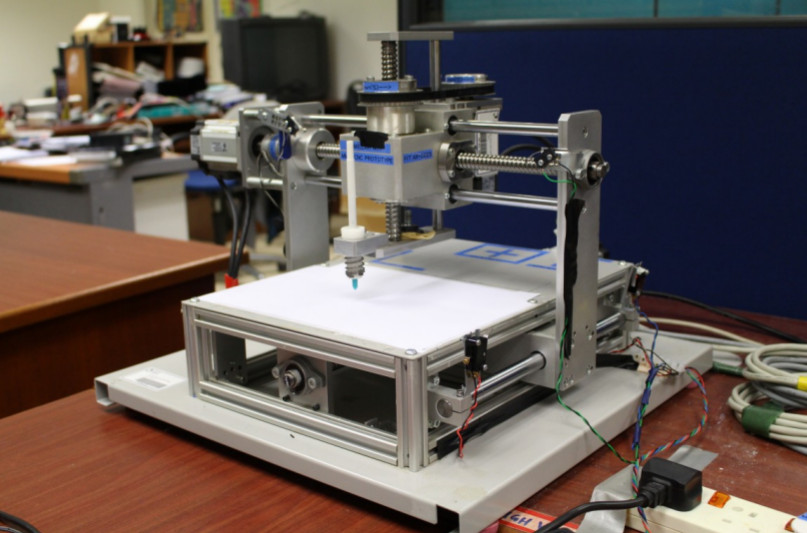
\includegraphics[width=0.85\textwidth]{./07-images/img-Ch4/CNC-Research-Machine-3-Axis.jpg}}
%%	\caption{The UMP 3-axis CNC Research Machine}
%%	\label{fig:CNC-Research-Machine-3-Axis.jpg}
%% \end{center}
%% \end{figure}

Electrical signal pulses sent to the servo-driver provide information like rotate clockwise (CW), rotate counter-clockwise(CCW), travel distance to rotate, speed to rotate, and so on. The actuation using electrical pulses makes the physical CNC machine instantaneously active. 




% ================== END CHAPTER-5 ========================